\documentclass[cal1spr16Lectures.tex]{subfiles}

\begin{document}

\section[]{}

% % %
\subsection[5.4 Working with Integrals]{\S 5.4 Working with Integrals}
% % %

% % %
\begin{frame}{\S 5.4 Working with Integrals}
Now that we have methods to use in integrating functions, we can examine applications of integration.  These applications include:
\begin{itemize}
\item Integration of even and odd functions;
\item Finding the average value of a functions;
\item Developing the Mean Value Theorem for Integrals.
\end{itemize}
\end{frame}

% % %
\subsubsection{Integrating Even and Odd Functions}
% % %
\begin{frame}{\small Integrating Even and Odd Functions}\small
Recall the definition of an even function,
\[f(-x)=f(x),\] 
and of an odd function, 
\[f(-x)=-f(x).\]

These properties simplify integrals when the interval in question is centered at the origin.
\end{frame}
%
% % %
%\subsubsection{Integrating Even Functions}
% % %

% % %
\begin{frame}%\footnotesize
Even functions are symmetric about the $y$-axis.  So 
%
%\vspace{-0.5pc}
\[
\int_{-a}^0 f(x)\ dx = \int_0^a f(x)\ dx
\]
%
%\vspace{-0.4pc}
i.e., the area under the curve to the left of the $y$-axis is equal to the area under the curve to the right.
\end{frame}

% % %
\begin{frame}
%\vspace{-1.1pc}
\begin{center}
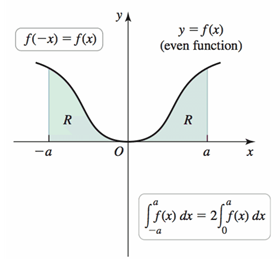
\includegraphics[scale=1]{pictures/Fig5_50a}
\end{center}
%
%Hence, $\int_{-a}^a f(x)\ dx = 2\int_0^a f(x)\ dx$ for even functions.
\end{frame}
%
% % %
%\subsubsection{Integrating Odd Functions}
% % %

% % %
\begin{frame}%{\small Integrating Odd Functions}
On the other hand, odd functions have $180^{\circ}$ rotation symmetry about the origin.  So
%
%\vspace{-1.25pc}
\[ 
\int_{-a}^0 f(x)\ dx = -\int_0^a f(x)\ dx
\]
%
%\vspace{-0.3pc}
i.e., the area under the curve to the left of the origin is the negative of the area under the curve to the right of the origin.
\end{frame}

% % %
\begin{frame}
%Hence, $\int_{-a}^a f(x)\ dx = 0$ for odd functions.
%\vspace{-0.6pc}
\begin{center}
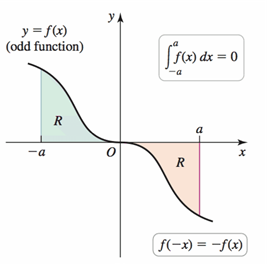
\includegraphics[scale=1]{pictures/Fig5_50b}
\end{center}
\end{frame}

% % %
\begin{frame}%[t]
\begin{exe}Evaluate the following integrals using the properties of even and odd functions:

\begin{itemize}

\vspace{0.25pc}
\item[(1)] $\int_{-4}^4 (3x^2-x)\ dx$

\vspace{0.5pc}
\item[(2)] $\int_{-1}^1 (1-|x|)\ dx$

\vspace{0.5pc}
\item [(3)] $\int_{-\pi}^{\pi} \sin x \ dx$
\end{itemize}
\end{exe}
\end{frame}

% % %
\subsubsection{Average Value of a Function}
% % %

% % %
\begin{frame}{\small Average Value of a Function}\footnotesize
Finding the average value of a function is similar to finding the average of a set of numbers.  We can estimate the average of $f(x)$ between points $a$ and $b$ by partitioning the interval $[a,b]$ into $n$ equally sized sections and choosing $y$-values $f(\overline{x}_k)$ for each $[x_{k-1},x_k]$.  The average is approximately  
%\[\frac{f(\overline{x}_1) + f(\overline{x}_2) + \dots + f(\overline{x}_n)}{n}\]
%Since $n=\dfrac{b-a}{\Delta x}$, we have
\begin{alignat*}{2}
\frac{f(\overline{x}_1) + f(\overline{x}_2) + \dots + f(\overline{x}_n)}{n} &= 
\frac{f(\overline{x}_1) + f(\overline{x}_2) + \dots + f(\overline{x}_n)}{\left(\frac{b-a}{\Delta x}\right)} \\
&= \frac{1}{b-a} \left(f(\overline{x}_1) + f(\overline{x}_2) + \dots + f(\overline{x}_n) \right) \Delta x \\
 &= \frac{1}{b-a}\sum_{k=1}^nf(\overline{x}_k)\Delta x
\end{alignat*}
\end{frame}

% % %
\begin{frame}{\small Average Value of a Function}\footnotesize
The estimate gets more accurate, the more $y$-values we take.  Thus the average value of an integrable function $f$ on the interval $[a,b]$ is 
\begin{align*}
\overline{f} &= \lim_{n\to \infty}\left(\frac{1}{b-a}\sum_{k=1}^nf(\overline{x}_k)\Delta x\right) \\
	&= \frac{1}{b-a}\left(\lim_{n\to\infty}\sum_{k=1}^nf(\overline{x}_k)\Delta x\right) \\
	&= \alert{\frac{1}{b-a} \int_a^b f(x)\ dx}.
\end{align*}
\end{frame}

% % %
\begin{frame}\small
\begin{ex}
The elevation of a path is given by $f(x)=x^3-5x^2+10$, where $x$ measures horizontal distances.  Draw a graph of the elevation function and find its average value for $0\leq x\leq 4$.
\end{ex}
\begin{exe} 
Find the average value of the function $f(x)=x(1-x)$ on the interval $[0,1]$. 
\end{exe}
\end{frame}

% % %
\subsubsection{Mean Value Theorem for Integrals}
% % %

% % %
\begin{frame}{\small Mean Value Theorem for Integrals}\footnotesize
The average value of a function leads to the Mean Value Theorem for Integrals.  Similar to the Mean Value Theorem from \S 4.6, the MVT for integrals says we can find a point $c$ between $a$ and $b$ so that $f(c)$ is the average value of the function.
\begin{thm}[Mean Value Theorem for Integrals] 
If $f$ is continuous on $[a,b]$, then there is at least one point $c$ in $[a,b]$ such that 
\[f(c)=\overline{f}=\frac{1}{b-a} \int_a^b f(x)\ dx.\]
\end{thm}
In other words, the horizontal line $y=\overline{f}=f(c)$ intersects the graph of $f$ for some point $c$ in $[a,b]$. 
\end{frame}

% % %
\begin{frame}
\begin{exe} 
Find or approximate the point(s) at which $f(x)=x^2-2x+1$ equals its average value on $[0,2]$. 
\end{exe}
\end{frame}

% % %
\subsubsection{Book Problems}
% % %

% % %
\begin{frame}
\begin{block}{5.4 Book Problems}
7-27 (odds), 31-39 (odds)
\end{block}
\end{frame}

\end{document}